%==============================================================================
% SECTION: Coherence as Layered Invariant
% Insert after Section 6 (Governance as Control System) or before Threat Model
%==============================================================================

\section{Coherence as Layered Invariant}
\label{sec:coherence-layers}

The term \emph{coherence} appears across multiple domains in distributed systems, from quantum physics to machine learning to governance. This section clarifies how procedural coherence ($\gamma$) relates to these other usages and argues that coherence preservation is a unifying principle across the full system stack.

\subsection{Three Layers of Coherence}

We identify three distinct but related coherence concepts:

\begin{definition}[Quantum Coherence]
In quantum information systems, coherence refers to the preservation of phase relationships between quantum states. A quantum channel maintains coherence when superposition states survive transmission without collapsing into classical mixtures. Formally, for density matrix $\rho$:
\[
\mathcal{C}_q(\rho) = \sum_{i \neq j} |\rho_{ij}|
\]
measures the off-diagonal elements that encode quantum correlations. Decoherence---the loss of these correlations through environmental interaction---degrades channel capacity and security guarantees in protocols like QKD.
\end{definition}

\begin{definition}[Geometric Coherence]
In representation learning and neural architectures, coherence refers to the preservation of semantic relationships in embedding spaces. A model maintains geometric coherence when:
\begin{enumerate}
    \item Similar inputs map to proximate regions of the embedding manifold
    \item Semantic operations (analogy, composition) correspond to geometric operations
    \item The manifold structure remains stable under perturbation
\end{enumerate}
Geometric incoherence manifests as embedding drift, manifold collapse, or semantic inconsistency---conditions where the model's internal representations no longer faithfully encode the relationships they purport to represent.
\end{definition}

\begin{definition}[Procedural Coherence]
In governance systems, coherence refers to the statistical properties of decision processes that indicate authentic, independent participation. As defined in Section~\ref{sec:pipeline}, the procedural coherence score:
\[
\gamma = \frac{\sigma^2_\eta}{255} \times 100
\]
measures entropy-weighted variance in voting patterns. Low $\gamma$ indicates coordinated behavior inconsistent with independent decision-making.
\end{definition}

\subsection{The Coherence Stack}

These three coherence types form a dependency hierarchy in systems that span physical infrastructure through algorithmic mediation to collective decision-making:

\begin{figure}[h]
\centering
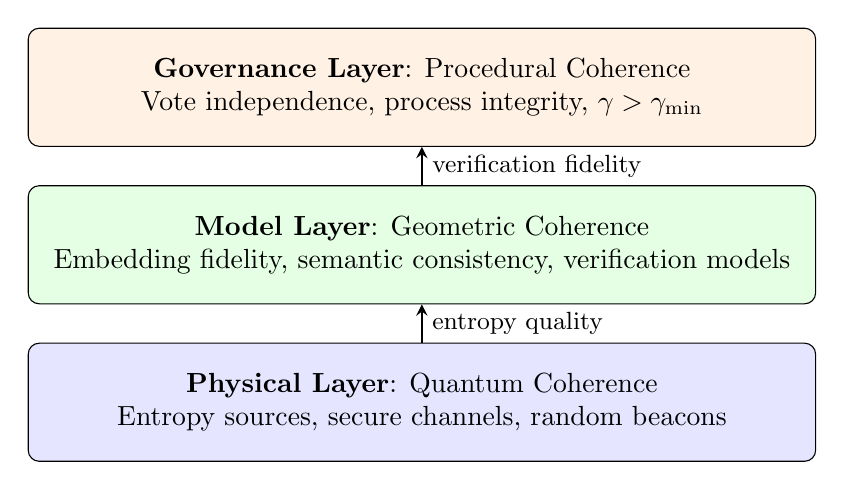
\begin{tikzpicture}[
    layer/.style={rectangle, draw, rounded corners, minimum width=10cm, minimum height=1.5cm, align=center},
    arrow/.style={->, thick, >=stealth}
]
\node[layer, fill=blue!10] (phys) at (0,0) {\textbf{Physical Layer}: Quantum Coherence\\Entropy sources, secure channels, random beacons};
\node[layer, fill=green!10] (model) at (0,2) {\textbf{Model Layer}: Geometric Coherence\\Embedding fidelity, semantic consistency, verification models};
\node[layer, fill=orange!10] (gov) at (0,4) {\textbf{Governance Layer}: Procedural Coherence\\Vote independence, process integrity, $\gamma > \gamma_{\min}$};

\draw[arrow] (phys) -- node[right, font=\small] {entropy quality} (model);
\draw[arrow] (model) -- node[right, font=\small] {verification fidelity} (gov);
\end{tikzpicture}
\caption{The coherence stack: each layer depends on coherence preservation in layers below.}
\label{fig:coherence-stack}
\end{figure}

\textbf{Physical $\to$ Model}: The entropy injection mechanism ($\epsilon \sim \pm 10\%$) that enables procedural coherence detection relies on high-quality randomness. If quantum entropy sources suffer decoherence, the resulting pseudo-randomness may exhibit patterns that either (a) fail to distinguish authentic from coordinated voting, or (b) introduce false positives by injecting correlated noise. Quantum coherence in the entropy generation layer is thus a precondition for meaningful $\gamma$ measurement.

\textbf{Model $\to$ Governance}: If test grid verification or artifact validation employs machine learning models (e.g., for semantic relevance checking, engagement verification, or anomaly detection), geometric coherence in those models affects governance outcomes. A model with collapsed embeddings may fail to distinguish substantively different proposals; a model with drifted representations may inconsistently apply admissibility criteria. Geometric coherence in the model layer is thus a precondition for consistent procedural application.

\subsection{Coherence Degradation Propagates Upward}

A critical property of the coherence stack is that degradation propagates upward but not downward:

\begin{proposition}[Upward Propagation]
Let $\mathcal{C}_q$, $\mathcal{C}_g$, and $\gamma$ denote quantum, geometric, and procedural coherence respectively. Then:
\[
\mathcal{C}_q < \mathcal{C}_q^{\min} \implies \mathbb{E}[\gamma] < \gamma_{\text{authentic}}
\]
and
\[
\mathcal{C}_g < \mathcal{C}_g^{\min} \implies \text{Var}[\gamma] > \text{Var}_{\text{expected}}
\]
That is, quantum decoherence biases procedural coherence measurements, and geometric incoherence increases their variance.
\end{proposition}

This has practical implications: a governance system cannot achieve reliable procedural coherence guarantees without monitoring coherence at lower layers. The $\gamma > 50$ threshold assumes baseline coherence in entropy sources and verification models.

\subsection{Unified Interpretation}

Despite domain-specific formalizations, all three coherence types share a common interpretation:

\begin{quote}
\emph{Coherence measures the degree to which a system preserves the structure it claims to preserve.}
\end{quote}

\begin{itemize}
    \item \textbf{Quantum}: Preserves superposition structure through transmission
    \item \textbf{Geometric}: Preserves semantic structure through embedding
    \item \textbf{Procedural}: Preserves independence structure through aggregation
\end{itemize}

In each case, coherence loss indicates that the system's outputs no longer faithfully represent its inputs according to the intended transformation. A decoherent quantum channel does not faithfully transmit quantum states; an incoherent embedding does not faithfully represent semantic relationships; an incoherent vote does not faithfully aggregate independent preferences.

\subsection{Implications for System Design}

The layered coherence model suggests several design principles:

\begin{enumerate}
    \item \textbf{Monitor all layers}: Governance coherence ($\gamma$) should be accompanied by monitoring of entropy source quality and model stability. Anomalies at lower layers may explain or predict governance-layer anomalies.

    \item \textbf{Establish layer-specific thresholds}: Just as $\gamma_{\min} = 50$ gates governance transitions, analogous thresholds should gate reliance on entropy sources ($\mathcal{C}_q^{\min}$) and verification models ($\mathcal{C}_g^{\min}$).

    \item \textbf{Fail safely on coherence loss}: When lower-layer coherence degrades, the system should either (a) halt governance operations, (b) fall back to higher-threshold requirements, or (c) switch to backup sources with intact coherence.

    \item \textbf{Audit coherence dependencies}: System audits should explicitly trace which coherence guarantees depend on which lower-layer assumptions, enabling targeted hardening.
\end{enumerate}

\subsection{Scope Clarification}

This paper focuses on procedural coherence ($\gamma$) and its role in governance integrity. The connections to quantum and geometric coherence are noted to:
\begin{enumerate}
    \item Clarify terminology for readers familiar with those domains
    \item Identify dependencies that affect $\gamma$ reliability
    \item Suggest a broader research program on coherence-preserving systems
\end{enumerate}

Full treatment of quantum coherence in entropy generation and geometric coherence in verification models is deferred to companion work. The procedural coherence results in this paper hold under the assumption that lower-layer coherence is maintained above implementation-specific thresholds.
